\documentclass[11pt]{article}

% ---------------------------------------------------------------------------
% Condensed preprint derived from the Bachelor's thesis (Trabajo Fin de Grado):
% "On the Limits of Low-Frequency OHLCV Signals in Machine Learning-Driven
%  Portfolio Optimization", J. Bengoechea Pardo, Universidad Politecnica de
%  Madrid, 2026. All numerical results are reproduced unchanged from the thesis.
%
% Build: bash build.sh   (or: latexmk -pdf main.tex; or upload paper/ to Overleaf)
% ---------------------------------------------------------------------------

\usepackage[margin=1in]{geometry}
\usepackage[utf8]{inputenc}
\usepackage[T1]{fontenc}
\usepackage{lmodern} % scalable fonts (required for microtype font expansion)
\usepackage{amsmath,amssymb}
\usepackage{booktabs}
\usepackage{graphicx}
\usepackage{microtype}
\usepackage[numbers,sort&compress]{natbib}
\usepackage[hidelinks]{hyperref}

\title{\textbf{On the Limits of Low-Frequency OHLCV Signals in\\
Machine Learning-Driven Portfolio Optimization}\\[0.4em]
\large A Cost-Aware, Leak-Free Benchmark on Large-Cap US Equities}

\author{Jaime Bengoechea Pardo\\
\small Escuela T\'ecnica Superior de Ingenieros Inform\'aticos\\
\small Universidad Polit\'ecnica de Madrid\\
\small \texttt{bengoecheapardo.jaime@gmail.com} \quad ORCID: 0009-0009-4387-5249}

\date{June 2026}

\begin{document}
\maketitle

\begin{abstract}
\noindent
The application of machine learning (ML) to quantitative finance has grown rapidly, yet
financial return series have an extremely low signal-to-noise ratio and are non-stationary,
exposing predictive pipelines to severe backtest overfitting. We conduct a rigorous, leak-free,
cost-aware stress-test of whether ML models trained only on monthly features derived from daily
OHLCV price and volume data can produce economically meaningful, net-of-cost portfolio
improvements over disciplined baselines, on a universe of 30 large-cap US equities (2010--2025).
A wide spectrum of models, namely regularized linear regressors, tree ensembles, and deep
networks (MLP, 1D-CNN, LSTM, CNN-LSTM, Transformer), is evaluated under an anchored
walk-forward scheme that retrains at each step, with a pre-specified promotion gate (mean
out-of-sample Spearman Rank IC $\ge 0.05$ on a 2016 hold-out) that admits only the MLP among the
deep models. Promoted forecasts enter a Black--Litterman optimizer as Bayesian views, with
Marchenko--Pastur covariance cleaning, dollar-neutral constraints, and realistic transaction
costs (10 bps). We report a negative result: in the out-of-sample period (2017--2025) the best
model (MLP, Sharpe 0.96) only marginally edges a no-ML Black--Litterman ``Prior-Only'' baseline
(Sharpe 0.94) that shares the same covariance cleaning, while incurring more than three times the
cumulative transaction cost (15.13\% vs.\ 4.67\%). More strikingly, a naive equally weighted
$1/30$ portfolio attains a Sharpe of 0.93, essentially tying the entire optimized apparatus.
Fama--French five-factor alphas of the active linear and tree strategies are statistically
insignificant. The risk-adjusted performance of the pipeline is driven by covariance
regularization and Bayesian shrinkage, expressed mainly as superior drawdown control, rather than
by the predictive content of the models. We release a fully reproducible pipeline as a baseline
for future studies.
\end{abstract}

\section{Introduction}
Under the Efficient Market Hypothesis \citep{fama1970efficient}, persistent excess returns from
public price information should be difficult to obtain in liquid markets. The modern financial
machine-learning literature \citep{gu2020empirical} has shown that flexible models can extract
non-linear, cross-sectional structure from large predictor sets, reviving the hope of systematic
alpha. Yet a large fraction of reported results is contaminated by data-snooping, look-ahead
leakage, and the omission of trading frictions \citep{lopezdeprado2018advances}. Reported Sharpe
ratios that ignore these issues routinely collapse out of sample, and the field suffers from a
publication bias toward positive findings. Careful negative results, which delimit where a
predictive edge does \emph{not} exist, are therefore valuable: they spare other researchers from
chasing exhausted signals.

This paper asks a deliberately narrow and answerable question:

\begin{quote}
\emph{Can machine-learning models trained exclusively on monthly features computed from daily
OHLCV price and volume data extract sufficient predictive alpha to generate statistically
significant and economically meaningful net-of-cost portfolio improvements in a highly efficient
large-cap equity universe, under institutional constraints and trading frictions?}
\end{quote}

Our hypothesis is that they cannot, and that the risk-adjusted benefits of a realistic pipeline
arise instead from robust covariance estimation and Bayesian shrinkage. We test this with an
end-to-end, leak-free, cost-aware benchmark and a strict, pre-registered model-promotion gate
that prevents non-predictive models from ever reaching the backtest. The design choices are made
to be conservative: a highly efficient large-cap universe (a hard test for any technical signal),
realistic transaction costs and slippage, anchored walk-forward retraining, and a held-out
validation gate.

\paragraph{Contributions.}
\begin{enumerate}
  \item A leak-free, cost-aware benchmark showing that ML models trained solely on monthly
  OHLCV-derived features do not deliver economically meaningful, net-of-cost improvements over a
  no-view Black--Litterman baseline on large-cap US equities.
  \item A clean performance attribution: by comparing against a Prior-Only baseline that shares
  the covariance cleaning and optimizer but uses no ML views, and against a naive $1/30$
  portfolio, we isolate the source of risk-adjusted performance and show it stems from
  regularization and risk control, not prediction. This reinforces, in a modern ML setting, the
  classical results of \citet{chopra1993effect} and \citet{demiguel2009optimal}.
  \item A reusable methodological building block: a data-driven calibration of the
  Black--Litterman view-uncertainty matrix tied to the rolling Information Coefficient, coupled
  with a disciplined pre-backtest promotion gate.
  \item A reproducible open codebase and a frozen data snapshot, providing a baseline against
  which future studies using higher-frequency or alternative data can be measured directly.
\end{enumerate}

\section{Related Work}
\paragraph{Classical asset pricing and portfolio theory.}
Mean-variance optimization \citep{markowitz1952portfolio} is the foundation of quantitative
allocation but is notoriously sensitive to estimation error in expected returns and covariances.
\citet{chopra1993effect} show that errors in the mean vector dominate portfolio loss by an order
of magnitude relative to errors in the covariance, and \citet{demiguel2009optimal} find that a
naive $1/N$ portfolio is hard to beat out of sample once estimation error is accounted for. These
results motivate shrinkage and regularization rather than unconstrained optimization, and they
frame our own finding that a $1/30$ portfolio is highly competitive.

\paragraph{Bayesian allocation.}
The Black--Litterman model \citep{black1992global,he1999intuition} addresses mean-variance
instability by blending a market-implied equilibrium prior with subjective views in a Bayesian
update, shrinking extreme allocations toward the market portfolio. A persistent practical
difficulty is the specification of the view-uncertainty matrix $\Omega$, which controls how
strongly the views move the posterior away from the prior. We address this with a data-driven
calibration tied to the rolling skill of each model.

\paragraph{Random matrix theory.}
Empirical correlation matrices estimated from finite financial samples are dominated by noise.
\citet{laloux1999noise} apply the Marchenko--Pastur law \citep{marchenko1967distribution} to
separate informative eigenvalues from the noise bulk, yielding more stable covariance estimates
for optimization. We use this spectral cleaning as the covariance backbone shared by every
optimized strategy, which lets us attribute performance differences cleanly to the views alone.

\paragraph{Financial machine learning and leakage.}
\citet{gu2020empirical} provide a large-scale demonstration of ML for empirical asset pricing,
while \citet{lopezdeprado2018advances} catalogues the methodological pitfalls (leakage,
overfitting, and improper cross-validation) that inflate backtested performance. Our work sits in
this tradition but emphasizes a careful, negative, replicable benchmark with realistic execution
assumptions rather than a new positive claim.

\section{Data and Universe}
We study 30 large-cap, highly liquid US equities drawn from the S\&P~500 and spanning GICS
sectors, over 2010--2025. Daily OHLCV data and historical market capitalizations are ingested via
Yahoo Finance; the S\&P~500 index (\verb|^GSPC|) serves as the market benchmark, and the
Fama--French five-factor library \citep{famafrench2015five} supplies the factor returns and the
risk-free rate. Data are aligned to the NYSE trading calendar and resampled to monthly frequency.
The sample is split into an experimentation period (2010--2016, with 2016 held out for
validation) and an out-of-sample backtest (2017--2025).

\paragraph{Scope and survivorship.}
The universe is a fixed list of companies that are large-cap today, which introduces survivorship
bias. We treat this deliberately as a fixed-universe stress-test of technical signals rather than
a survivorship-free alpha-discovery study. The bias inflates all strategies comparably, so the
relative conclusion, namely that ML views add little over the Prior-Only baseline net of costs,
is robust. Absolute outperformance versus the index should be read as caveated, not as a
tradeable claim. Restricting the universe to 30 liquid blue chips also keeps a flat 10 bps cost
model realistic, since these names absorb institutional-size trades with minimal market impact.

\section{Methodology}

\subsection{Features and target}
For each asset and month we compute a panel of technical features from daily OHLCV bars. These
span six families: (i) returns and momentum across multiple horizons; (ii) intraday price-action
metrics derived from the open-high-low-close geometry; (iii) range-based volatility estimators
such as the Parkinson \citep{parkinson1980extreme} and Rogers--Satchell estimators; (iv) volume
and liquidity measures, including the Amihud illiquidity ratio \citep{amihud2002illiquidity};
(v) efficiency, persistence, and higher-moment statistics (skewness and kurtosis); and (vi)
CAPM-derived systematic and idiosyncratic components (rolling beta and residual alpha). The
prediction target is the next-month log-return,
\begin{equation}
Y_t = \ln\!\left(\frac{P_{t+1}}{P_t}\right).
\end{equation}

\subsection{Preprocessing and leakage control}
All cross-sectional preprocessing is fit on past data only. Features are winsorized at
cross-sectional quantiles to limit the influence of outliers, then standardized using rolling
statistics, so that no future information enters the scaling of any training sample. Highly
collinear features are pruned with variance-inflation-factor diagnostics to stabilize the linear
models and the covariance estimates. This discipline is the practical answer to the leakage
critique of \citet{lopezdeprado2018advances}: the entire pipeline is causal with respect to the
forecast boundary.

\subsection{Models}
We evaluate three model families. The linear family comprises ordinary least squares and its
regularized variants (Lasso, Ridge, ElasticNet), which are interpretable and naturally resistant
to overfitting in low signal-to-noise regimes. The tree family comprises Random Forest (bagging)
and XGBoost (gradient boosting \citep{chen2016xgboost}), which capture non-linear interactions.
The deep family comprises a multilayer perceptron (MLP), a 1D temporal CNN, an LSTM, a CNN-LSTM
hybrid, and a Transformer \citep{vaswani2017attention}. Networks are trained with the Huber loss
(robust to return outliers) and the AdamW optimizer under a cosine-annealing learning-rate
schedule.

\subsection{Walk-forward validation, hybrid retraining, and the promotion gate}
We use an anchored walk-forward scheme that retrains at each monthly step on an expanding window.
To control hyperparameter-search overfitting and computational cost, a high-dimensional Optuna
\citep{akiba2019optuna} search (tree-structured Parzen estimator with successive-halving pruning)
is run once per year, in December, and the chosen hyperparameters are then re-fit on the expanding
window during the intermediate months. This hybrid reduces compute by roughly 90\% relative to
monthly re-tuning while preserving out-of-sample integrity.

Before any model may enter the backtest, it must clear a pre-specified \emph{promotion gate}: a
mean out-of-sample Rank IC of at least $0.05$ on the 2016 hold-out window. The Information
Coefficient at month $t$ is the Spearman rank correlation between predicted returns
$\hat R_{i,t+1}$ and realized returns $R_{i,t+1}$ across the $N$ stocks, computed as the Pearson
correlation of their tie-corrected ranks,
\begin{equation}
\text{Rank IC}_t = \frac{\operatorname{cov}\!\big(\operatorname{rank}(\hat R_{\cdot,t+1}),\,
\operatorname{rank}(R_{\cdot,t+1})\big)}
{\sigma_{\operatorname{rank}(\hat R)}\,\sigma_{\operatorname{rank}(R)}},
\qquad
\overline{\text{IC}} = \frac{1}{T}\sum_{t=1}^{T}\text{Rank IC}_t .
\label{eq:ic}
\end{equation}
In the implementation, Eq.~\eqref{eq:ic} is evaluated with \texttt{scipy.stats.spearmanr} for the
shallow models and with an equivalent differentiable Pearson-on-ranks routine (using average-tie
ranks) for the neural networks, so that the same statistic drives both validation and the gate.
The threshold of $0.05$ reflects the fact that a cross-sectional IC in this range is a weak but
genuine signal in equity markets; models below it are presumed to carry no exploitable
information.

\subsection{Allocation: Black--Litterman with covariance cleaning}
Promoted forecasts enter the Black--Litterman model \citep{black1992global,he1999intuition} as
views $Q$. The posterior mean return vector is
\begin{equation}
\hat{\Pi} = \left[(\tau \Sigma)^{-1} + P^{\top} \Omega^{-1} P\right]^{-1}
            \left[(\tau \Sigma)^{-1} \Pi + P^{\top} \Omega^{-1} Q\right],
\end{equation}
where $\Pi$ is the market-implied equilibrium prior (from reverse optimization on market-cap
weights), $P$ the link matrix, and $\tau$ a prior-scaling parameter. The diagonal view-uncertainty
matrix $\Omega$ is calibrated dynamically from each model's rolling Rank IC: a higher recent IC,
with a higher signal-to-noise ratio across the IC history, produces lower view uncertainty and
therefore greater posterior weight on the model's views. This ties the confidence placed in a
model directly to its demonstrated out-of-sample skill. The covariance $\Sigma$ is cleaned with
random matrix theory: eigenvalues falling within the Marchenko--Pastur band
\citep{marchenko1967distribution,laloux1999noise},
\begin{equation}
\lambda_\pm = \sigma^2\Big(1 \pm \sqrt{N/T}\,\Big)^2,
\end{equation}
are treated as noise and replaced by their average, preserving total variance while removing
spurious correlation structure.

\subsection{Backtesting engine and baselines}
Portfolios are solved monthly under institutional constraints (dollar neutrality, a gross-leverage
cap of 2.0, and per-position bounds) using the ECOS conic solver \citep{domahidi2013ecos} in
CVXPY. Transaction costs are modeled at 10 bps (5 bps commission plus 5 bps slippage, in the
spirit of \citet{almgren2001optimal}), applied to traded turnover, with weight drift between
rebalances and a self-financing structure that yields net excess returns. We benchmark every
active strategy against five baselines: the S\&P~500 index; an equally weighted $1/30$ portfolio;
unregularized mean-variance optimization (MVO); the Prior-Only Black--Litterman portfolio (same
covariance cleaning and optimizer, no ML views); and a random-view control that injects pure noise
as views.

\subsection{Statistical evaluation}
Because overlapping monthly returns are autocorrelated and heteroskedastic, ordinary standard
errors are biased; we therefore report Newey--West HAC \citep{newey1987simple} $t$-statistics.
Risk-adjusted alpha is assessed with Fama--French five-factor regressions
\citep{famafrench2015five}, and path robustness with Politis--Romano stationary-bootstrap
\citep{politis1994stationary} Monte-Carlo simulation (10{,}000 resampled paths per strategy),
from which we read terminal-wealth, Sharpe, and drawdown distributions.

\section{Results}

\subsection{Promotion gate}
Among the deep models, only the MLP cleared the gate (mean Rank IC $0.061$); the CNN ($0.038$),
LSTM ($0.029$), CNN-LSTM ($0.040$), and Transformer ($0.029$) failed, consistent with overfitting
in a data-scarce panel and the absence of peak-validation checkpointing. The promoted set
therefore comprises the regularized linear models, the two tree ensembles, and the MLP.

\subsection{Headline performance}
Table~\ref{tab:results} summarizes the 2017--2025 backtest, and Figure~\ref{fig:curves} shows the
out-of-sample equity curves of the MLP and Prior-Only strategies. Three regularities stand out.

First, the optimized long-short strategies produce visually near-identical equity curves, because
every allocation is dominated by the same Marchenko--Pastur-cleaned covariance and the same
market-cap equilibrium prior; the ML views perturb, but do not reshape, these weights. The MLP and
Prior-Only curves in Figure~\ref{fig:curves} are almost indistinguishable.

Second, on a risk-adjusted basis the Prior-Only baseline (Sharpe 0.94) and the MLP (Sharpe 0.96)
lead, ahead of the passive S\&P~500 (0.72), while the individual linear and tree models cluster
well below (Sharpe 0.50 to 0.58), dragged down by the turnover their active views generate, and
the naive MVO portfolio collapses (Sharpe $-0.29$, a total return of $-22.47\%$). The active
machine-learning models never convincingly beat the no-model Prior-Only baseline net of costs, and
only the MLP edges it at all, by a slim and cost-eroded margin.

Third, and most tellingly, the equally weighted $1/30$ portfolio achieves a Sharpe of 0.93 and the
highest raw return in the study (323.41\%), essentially tying the entire optimized apparatus on a
risk-adjusted basis. This is a direct echo of \citet{demiguel2009optimal}: naive diversification
is extremely hard to beat. The optimized Black--Litterman strategies do retain one genuine
advantage, but it is in \emph{risk control}, not return: their maximum drawdowns ($-25.8\%$) are
markedly shallower than the fully market-exposed $1/30$ and index portfolios ($-34$ to $-36\%$),
and they are dollar-neutral with near-zero market beta rather than carrying a beta of 1.0.

\begin{table}[t]
\centering
\caption{Out-of-sample results (2017--2025), net of 10 bps transaction costs. Best value per
column in \textbf{bold}. ElasticNet, XGBoost, and Random Forest are shown as the representative
linear and tree models; the remaining linear models fall in the same 0.50--0.58 Sharpe cluster.}
\label{tab:results}
\small
\begin{tabular}{lccccc}
\toprule
Strategy & Cum.\ Return & CAGR & Sharpe & Sortino & Max Drawdown \\
\midrule
S\&P 500 Index            & 200.39\% & 13.00\% & 0.72 & 1.10 & $-33.92\%$ \\
Equally Weighted ($1/30$) & \textbf{323.41\%} & \textbf{17.39\%} & 0.93 & 1.50 & $-34.46\%$ \\
Mean-Variance (MVO)       & $-22.47\%$ & $-2.78\%$ & $-0.29$ & $-0.38$ & $-40.59\%$ \\
BL Prior-Only (No ML)     & 236.94\% & 14.45\% & 0.94 & 1.66 & $\mathbf{-25.80\%}$ \\
BL MLP (Active)           & 244.89\% & 14.75\% & \textbf{0.96} & \textbf{1.70} & $-25.82\%$ \\
BL ElasticNet (Active)    & 129.89\% & 9.70\% & 0.58 & 0.97 & $-25.16\%$ \\
BL XGBoost (Active)       & 126.31\% & 9.51\% & 0.55 & 0.93 & $-27.06\%$ \\
BL Random Forest (Active) & 109.21\% & 8.55\% & 0.50 & 0.81 & $-27.46\%$ \\
\bottomrule
\end{tabular}
\end{table}

\begin{figure}[t]
\centering
\begin{minipage}{0.49\textwidth}
  \centering
  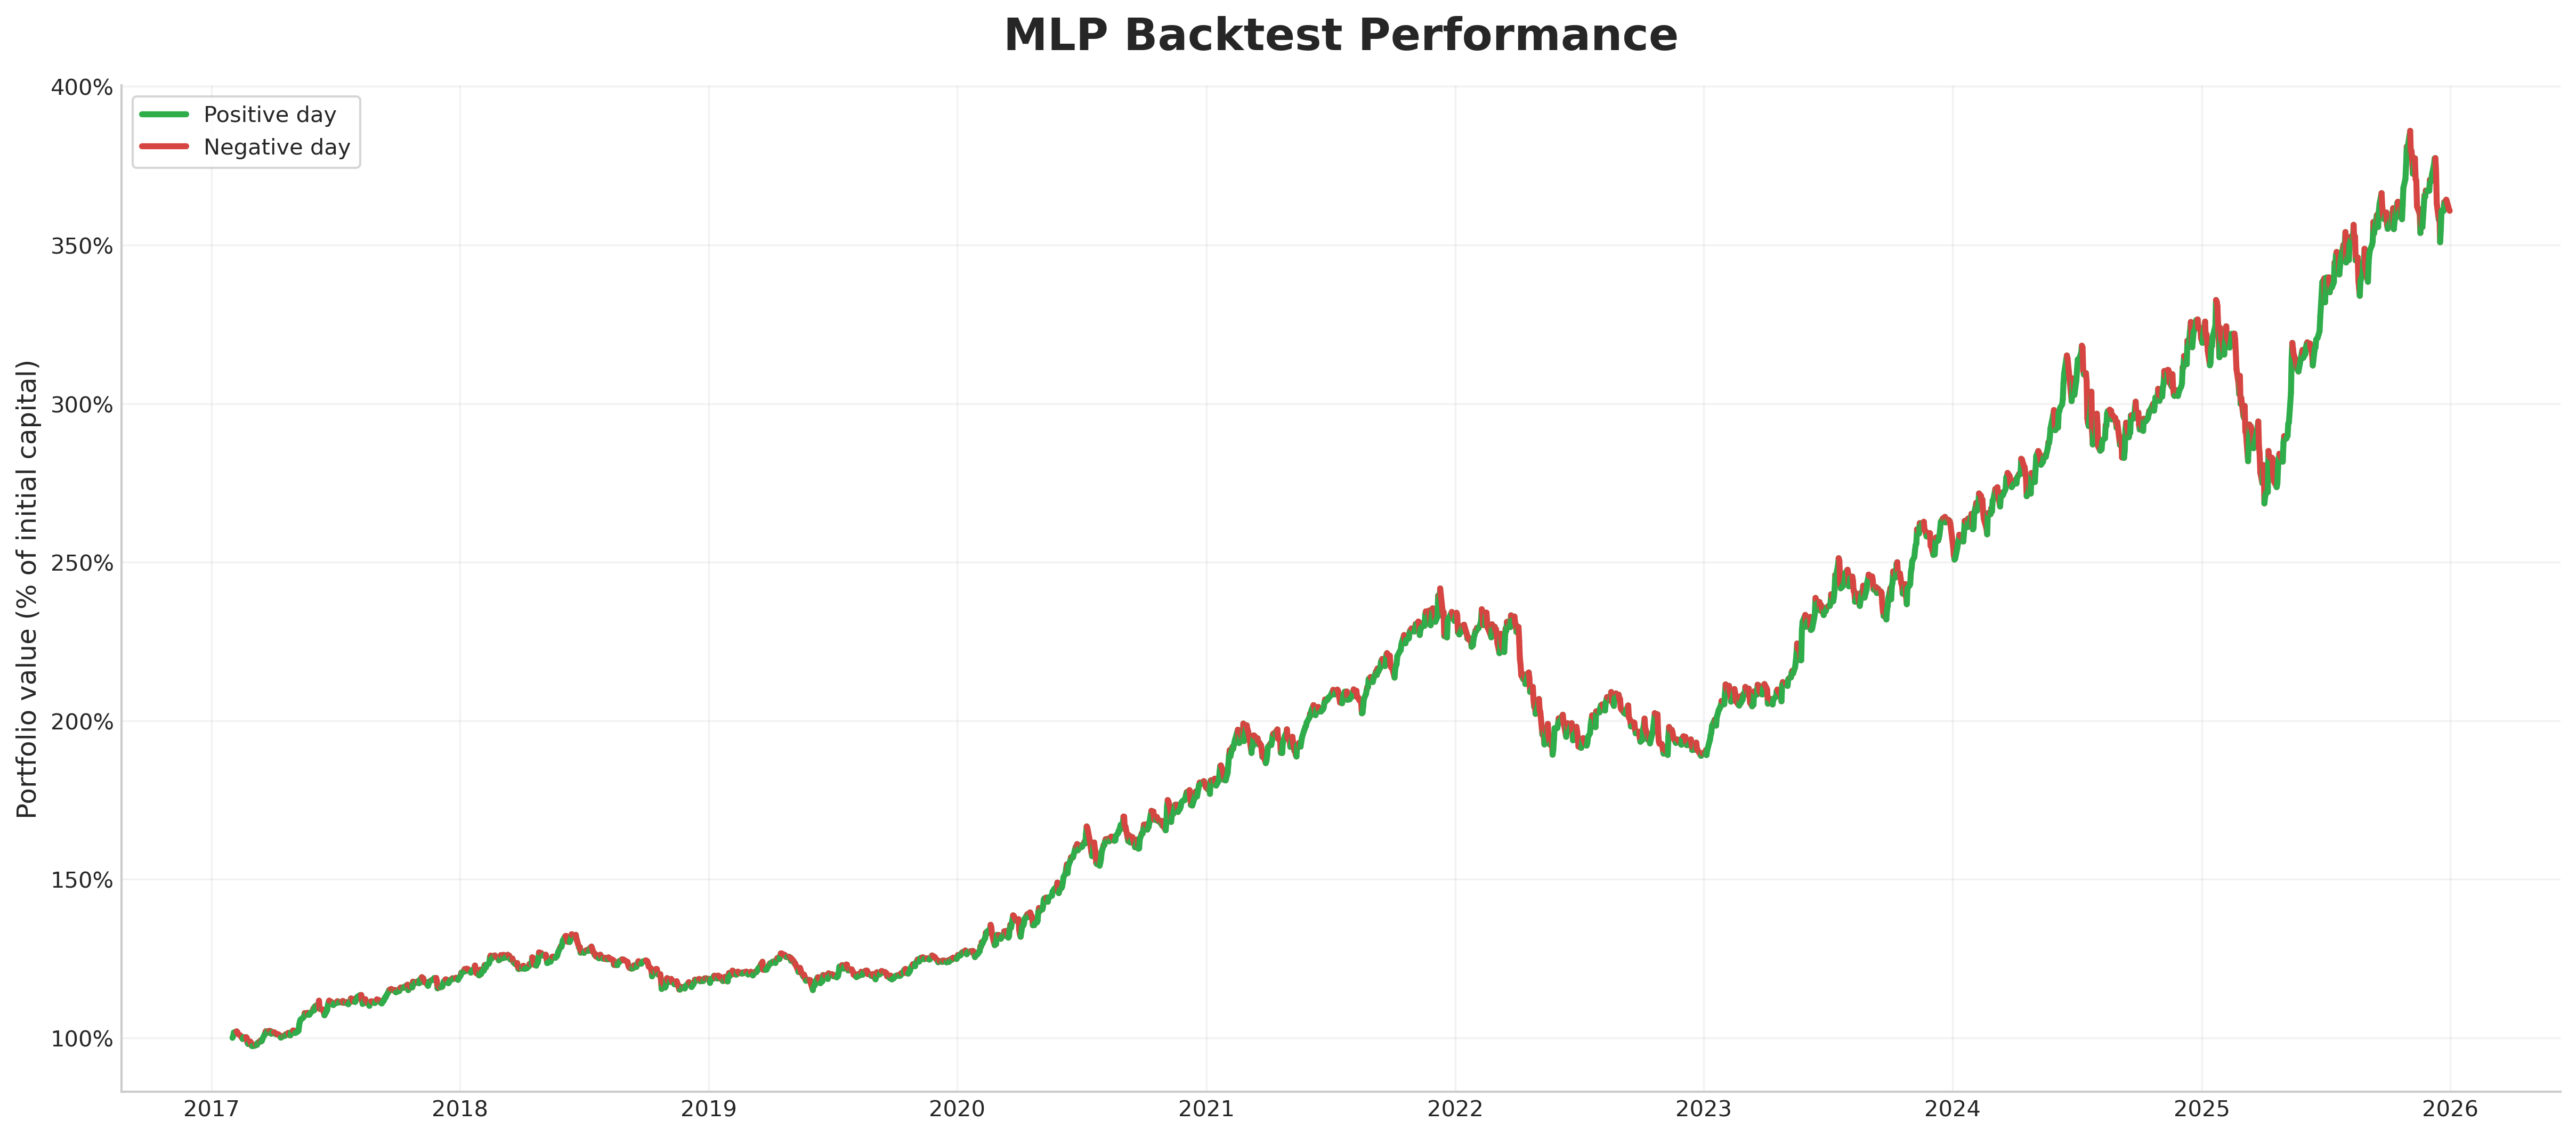
\includegraphics[width=\linewidth]{figs/mlp_backtest.png}\\
  {\small (a) BL-MLP (active ML views)}
\end{minipage}
\hfill
\begin{minipage}{0.49\textwidth}
  \centering
  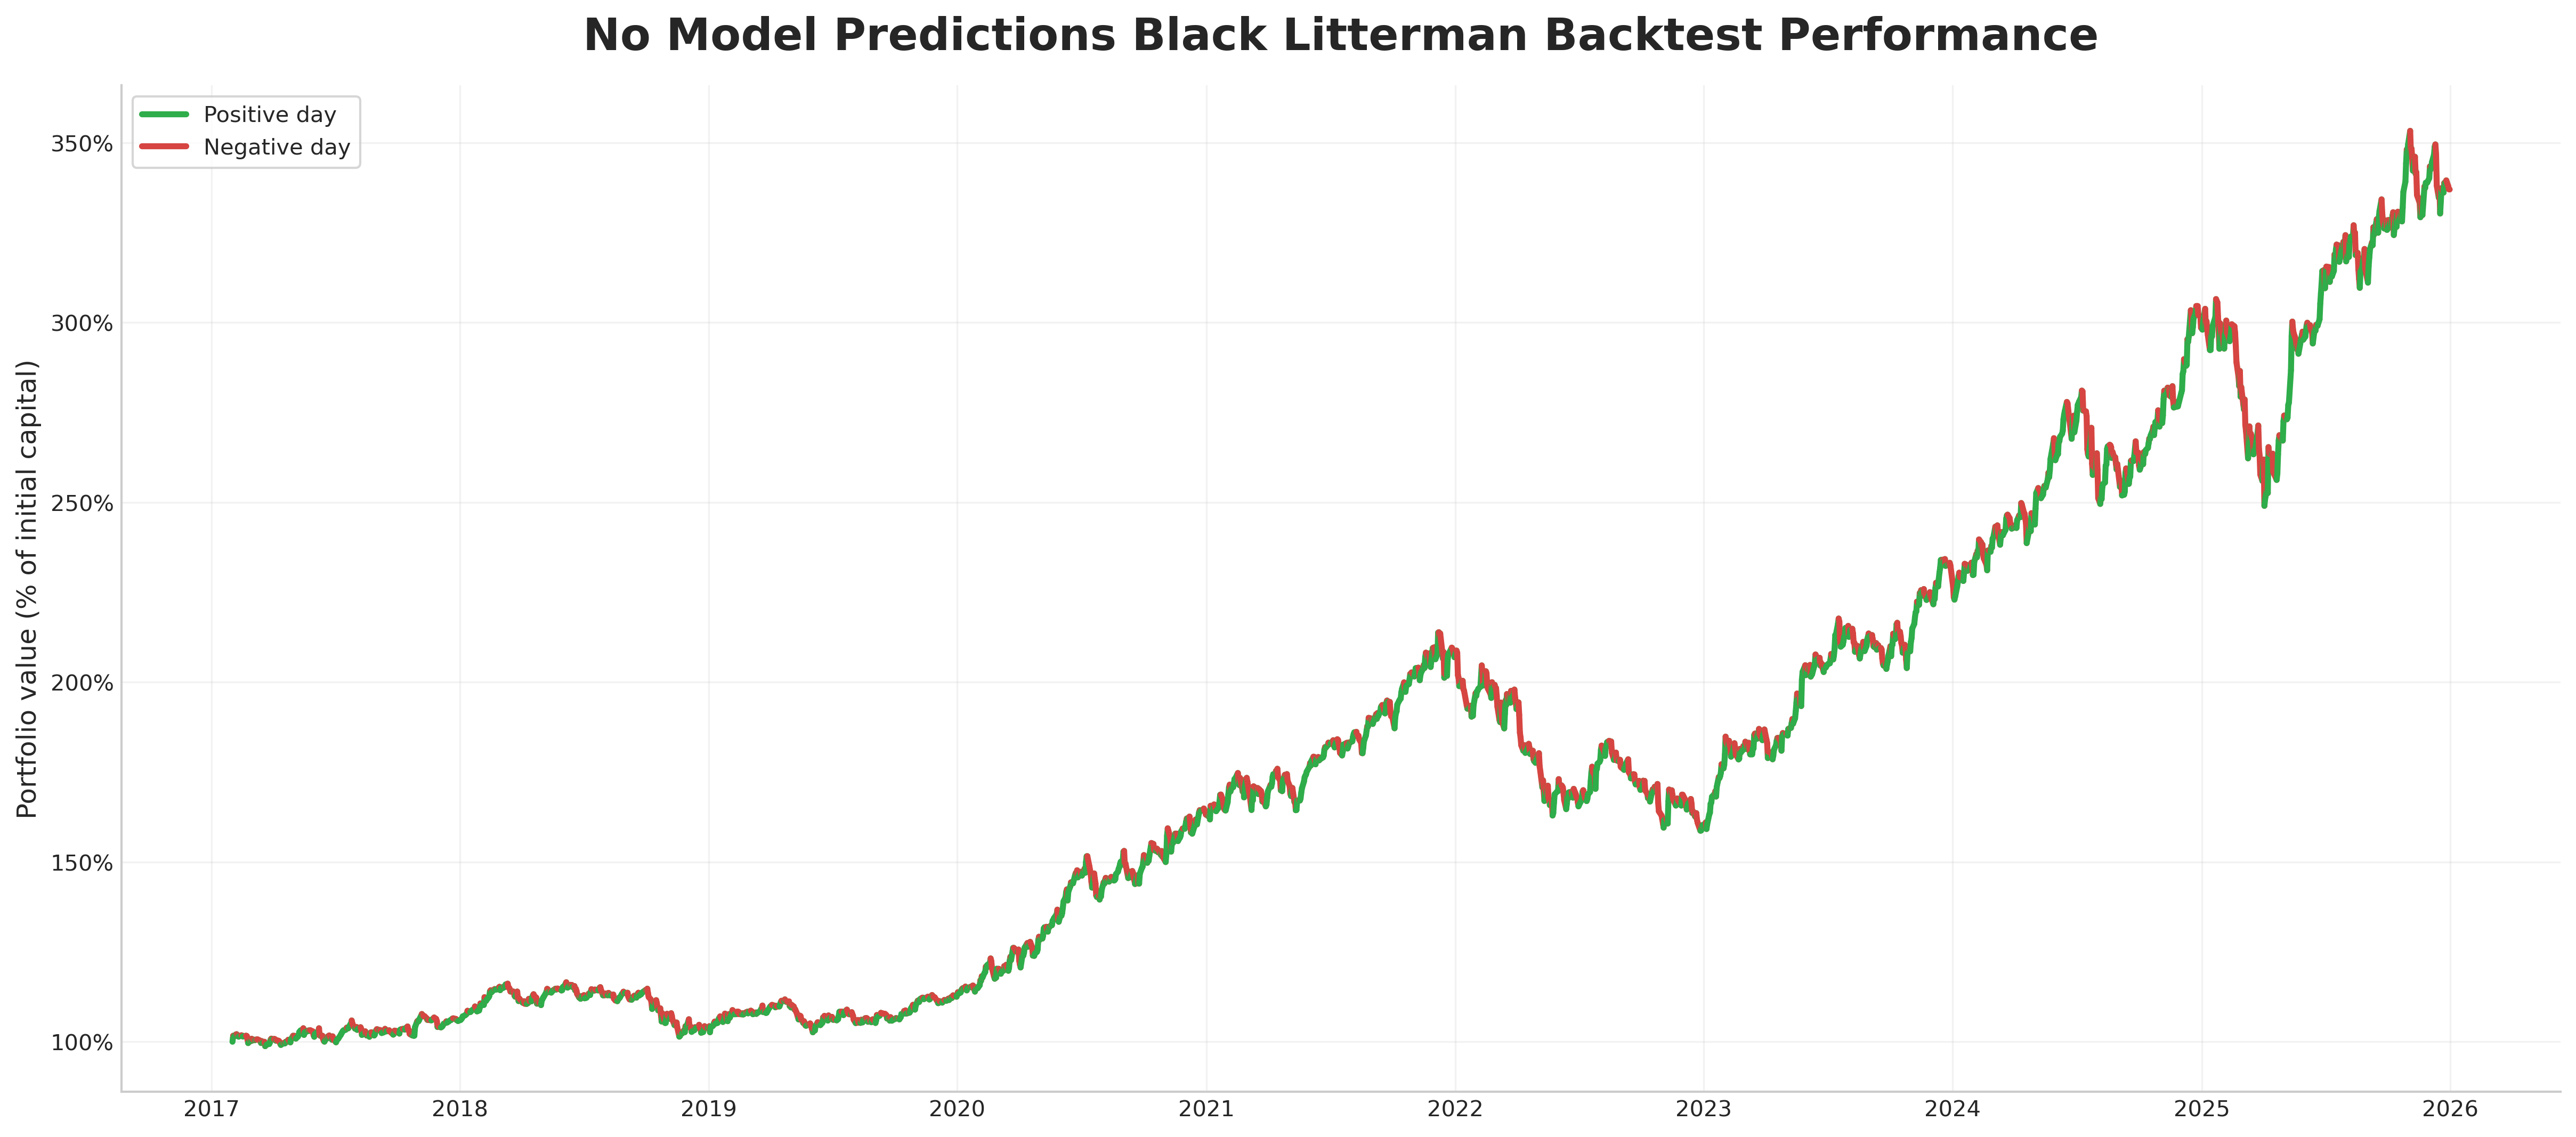
\includegraphics[width=\linewidth]{figs/prioronly_backtest.png}\\
  {\small (b) BL Prior-Only (no ML views)}
\end{minipage}
\caption{Out-of-sample cumulative performance (2017--2025), as a percentage of initial capital.
The active-ML (a) and no-ML (b) portfolios trace nearly identical paths, illustrating that the
risk-management layer, not the ML views, drives the result. See Table~\ref{tab:results} for the
full comparison.}
\label{fig:curves}
\end{figure}

\subsection{The decisive role of transaction costs}
Costs explain why the active models underperform the Prior-Only baseline. The Prior-Only portfolio
trades slowly and accumulates only 4.67\% in cumulative transaction costs over the period, whereas
the MLP, whose active views drive much higher turnover, accumulates 15.13\%, and XGBoost is the
most expensive strategy in the study at 17.46\%. The $1/30$ portfolio trades cheaply by
construction. The active models' gross predictive edge, already small, is therefore almost
entirely eroded by trading friction, leaving net Sharpe ratios in the 0.50 to 0.58 range for the
individual linear and tree models.

\subsection{Statistical significance and factor attribution}
HAC-adjusted $t$-statistics of net return drifts are significant for Prior-Only (3.26), MLP
(3.19), and Equally-Weighted (4.18), but fall to the 1.8 to 2.1 range for the individual linear
and tree models, so their net returns are only weakly distinguishable from zero. The Fama--French
five-factor regressions tell the same story: the annualized alphas of the linear and tree
strategies (2 to 3\%) carry $p$-values around 0.5 to 0.7 and are statistically insignificant,
meaning none delivers risk-adjusted return beyond passive factor exposure. The active models load
on a small positive market beta (about 0.32 to 0.35) with negative value and investment tilts, a
near-uniform factor fingerprint across the whole active cohort.

\subsection{Where the performance comes from}
Because the Prior-Only baseline shares the covariance cleaning and the optimizer but uses no ML
views, its near-identical risk-adjusted performance localizes the source of utility to the
risk-management layer (Marchenko--Pastur cleaning and Black--Litterman shrinkage) rather than to
model prediction. Two further controls sharpen this. The MLP's cross-sectional Model IC decays
from about $0.06$ in validation to about $0.02$ live, confirming that the residual edge is small
and unstable. And the random-view control, which feeds pure noise into the same optimizer, still
produces positive returns: it establishes a noise floor showing that the apparatus makes money
from risk management even when the views contain no information whatsoever.

\subsection{Monte-Carlo robustness}
The stationary bootstrap corroborates the point-estimate reading. The Sharpe-ratio distributions
of the active models overlap heavily with that of the Prior-Only baseline, and the wide dispersion
of terminal-wealth cones overwhelms the small differences in their centres. No active model
converts its nominal point-estimate lead into a reliably repeatable edge across resampled paths.

\section{Discussion: Practical Implications}
Beyond the headline finding, the study yields two practitioner-facing lessons. First, on
methodology: the gap between the gross and net performance of the active models is a concrete
demonstration that backtests omitting realistic turnover and transaction costs are misleading, and
that a pre-specified promotion gate is an effective, cheap guard against advancing non-predictive
models into an expensive backtest. The same architecture that reports a high Sharpe on paper can
be revealed as cost-dominated once friction and a held-out skill check are imposed. For allocators,
the operational implication is that robust covariance estimation and disciplined shrinkage deliver
most of the realisable utility, and are far more reliable than a marginal, unstable forecasting
edge.

Second, on computational cost: the hybrid retraining scheme, which restricts the expensive Optuna
hyperparameter search to an annual cadence while re-fitting parameters monthly on the expanding
window, reduces compute (and the associated energy use) by roughly 90\% relative to retuning at
every rebalance, with no loss of out-of-sample integrity. In an era of growing scrutiny of the
energy footprint of machine learning, this is a practical template for keeping rolling
walk-forward research tractable and efficient without compromising methodological rigour.

\section{Limitations}
The universe is small (30 names), US large-cap, and monthly: the most informationally efficient
regime, and not generalizable to small-caps or higher frequencies. The fixed universe carries
survivorship bias, bounded in Section~3. The deep-model outcome is partly capacity-bound and
implementation-bound: the panel (about 2{,}160 observations) is data-scarce for sequential
networks, and training lacked peak-validation early-stopping checkpointing, so the result should
be read as ``not supported in this setup'' rather than as a general impossibility. The promotion
gate uses a single hold-out year.

\section{Future Work}
The natural extensions follow directly from these limitations. Higher-frequency limit-order-book
data would capture microstructure dynamics (order-flow imbalance, spread variation) that monthly
bars smooth away, and would invite continuous-time tools such as Hawkes processes and stochastic
differential equations. Broadening the predictor space to macroeconomic series and alternative
data (news and filings sentiment) could resolve cross-sectional dispersion that price-only
features miss. Expanding the universe to the full S\&P~500 or Russell~3000 over several decades
would supply the sample sizes that deep sequential models require, paired with proper
EMA-IC-based early stopping. Finally, moving from point forecasts to predictive distributions
(quantile or mixture-density models) would allow tail-risk-aware optimization and an end-to-end
Monte-Carlo stress test that re-generates signals and re-runs the optimizer on each path.

\section{Conclusion}
On large-cap US equities at monthly frequency, features computed from daily OHLCV data carry a
signal too weak and unstable to generate robust, cost-justified alpha. A disciplined pipeline
still produces attractive risk-adjusted performance, but that performance is driven by covariance
regularization and Bayesian shrinkage, expressed as superior drawdown control, not by ML
prediction; indeed a naive $1/30$ portfolio ties the optimized strategies on Sharpe. Documenting
this negative result carefully, with realistic costs and a pre-registered gate, is the
contribution: it marks where a predictive edge is not found, and provides a reproducible baseline
for studies using higher-frequency, alternative, or macro data.

\section*{Reproducibility}
The complete pipeline, a frozen data snapshot, and the full thesis are archived with a permanent
DOI, and the code is released under the MIT license. The global random seed is fixed; because
Yahoo Finance adjusted prices are recomputed on later corporate actions, exact reproduction
requires the frozen snapshot rather than a fresh download. See the repository \texttt{README} and
\texttt{DATASET.md} for details.

\section*{Acknowledgements}
This work is the author's Bachelor's thesis at Universidad Polit\'ecnica de Madrid, supervised by
Antonio Garc\'ia Dopico (DATSI). Generative AI was used only for literature search; all code and
derivations are the author's own.

\bibliographystyle{unsrtnat}
\bibliography{references}

\end{document}
